% 1章
\chapter{序論}
\label{chap:introduction}
%
%\input{introduction/preface}
%
%!TEX root = ../thesis.tex

\section{背景}
AIFormulaは計測自動制御学会と自動車技術会が主催し, 本田技術研究所がサポートする次世代の人工知能モビリティの競技会で, 正式な競技会は2025年から始まる.
AIFormulaは今後ますます需要が高まるであろう自動化システムの技術者を育てるという点で効果が見込まれる.
AIFormulaではハードウェアの変更もある程度許容されているが, 現時点での開発はソフトウェアが中心となる.
ハードウェアは経路追従するために必要なパーツが全て揃っているが, ソフトウェアはデバイスを駆動するサンプルプログラムが用意されているのみである.
競技という性質上, 経路追従などのソフトウェアは各チームで開発することが必要となる.
その点で, コースを自動で走行するためにはソフトウェアの開発は必須となる.

\subsection{ハードウェアとルール}
AIFormulaでは詳細なルールは検討中であるとのことで, 2025年2月に開催される予定のプレ大会以降に詳細なルールが決定される予定となっている.
Fig.1に2025年のプレ大会で使用されるロボットを示す.
プレ大会では指定されたコースを3周する時間で競われる.
LiDARなどは使用できないなど, いくつかの制約がある.

\begin{figure}[H]
  \centering
 \includegraphics[keepaspectratio, scale=0.6]
      {images/ExteriorViewOfTheMobilityPlatform.png}
 \caption{Exterior view of the mobility platform}
 \label{fig:robot view}
\end{figure}

\subsection{コース}
Fig.2にAIFormulaのコースを示す.
周囲に高い建造物のない平坦なコースである.


\begin{figure}[H]
  \centering
 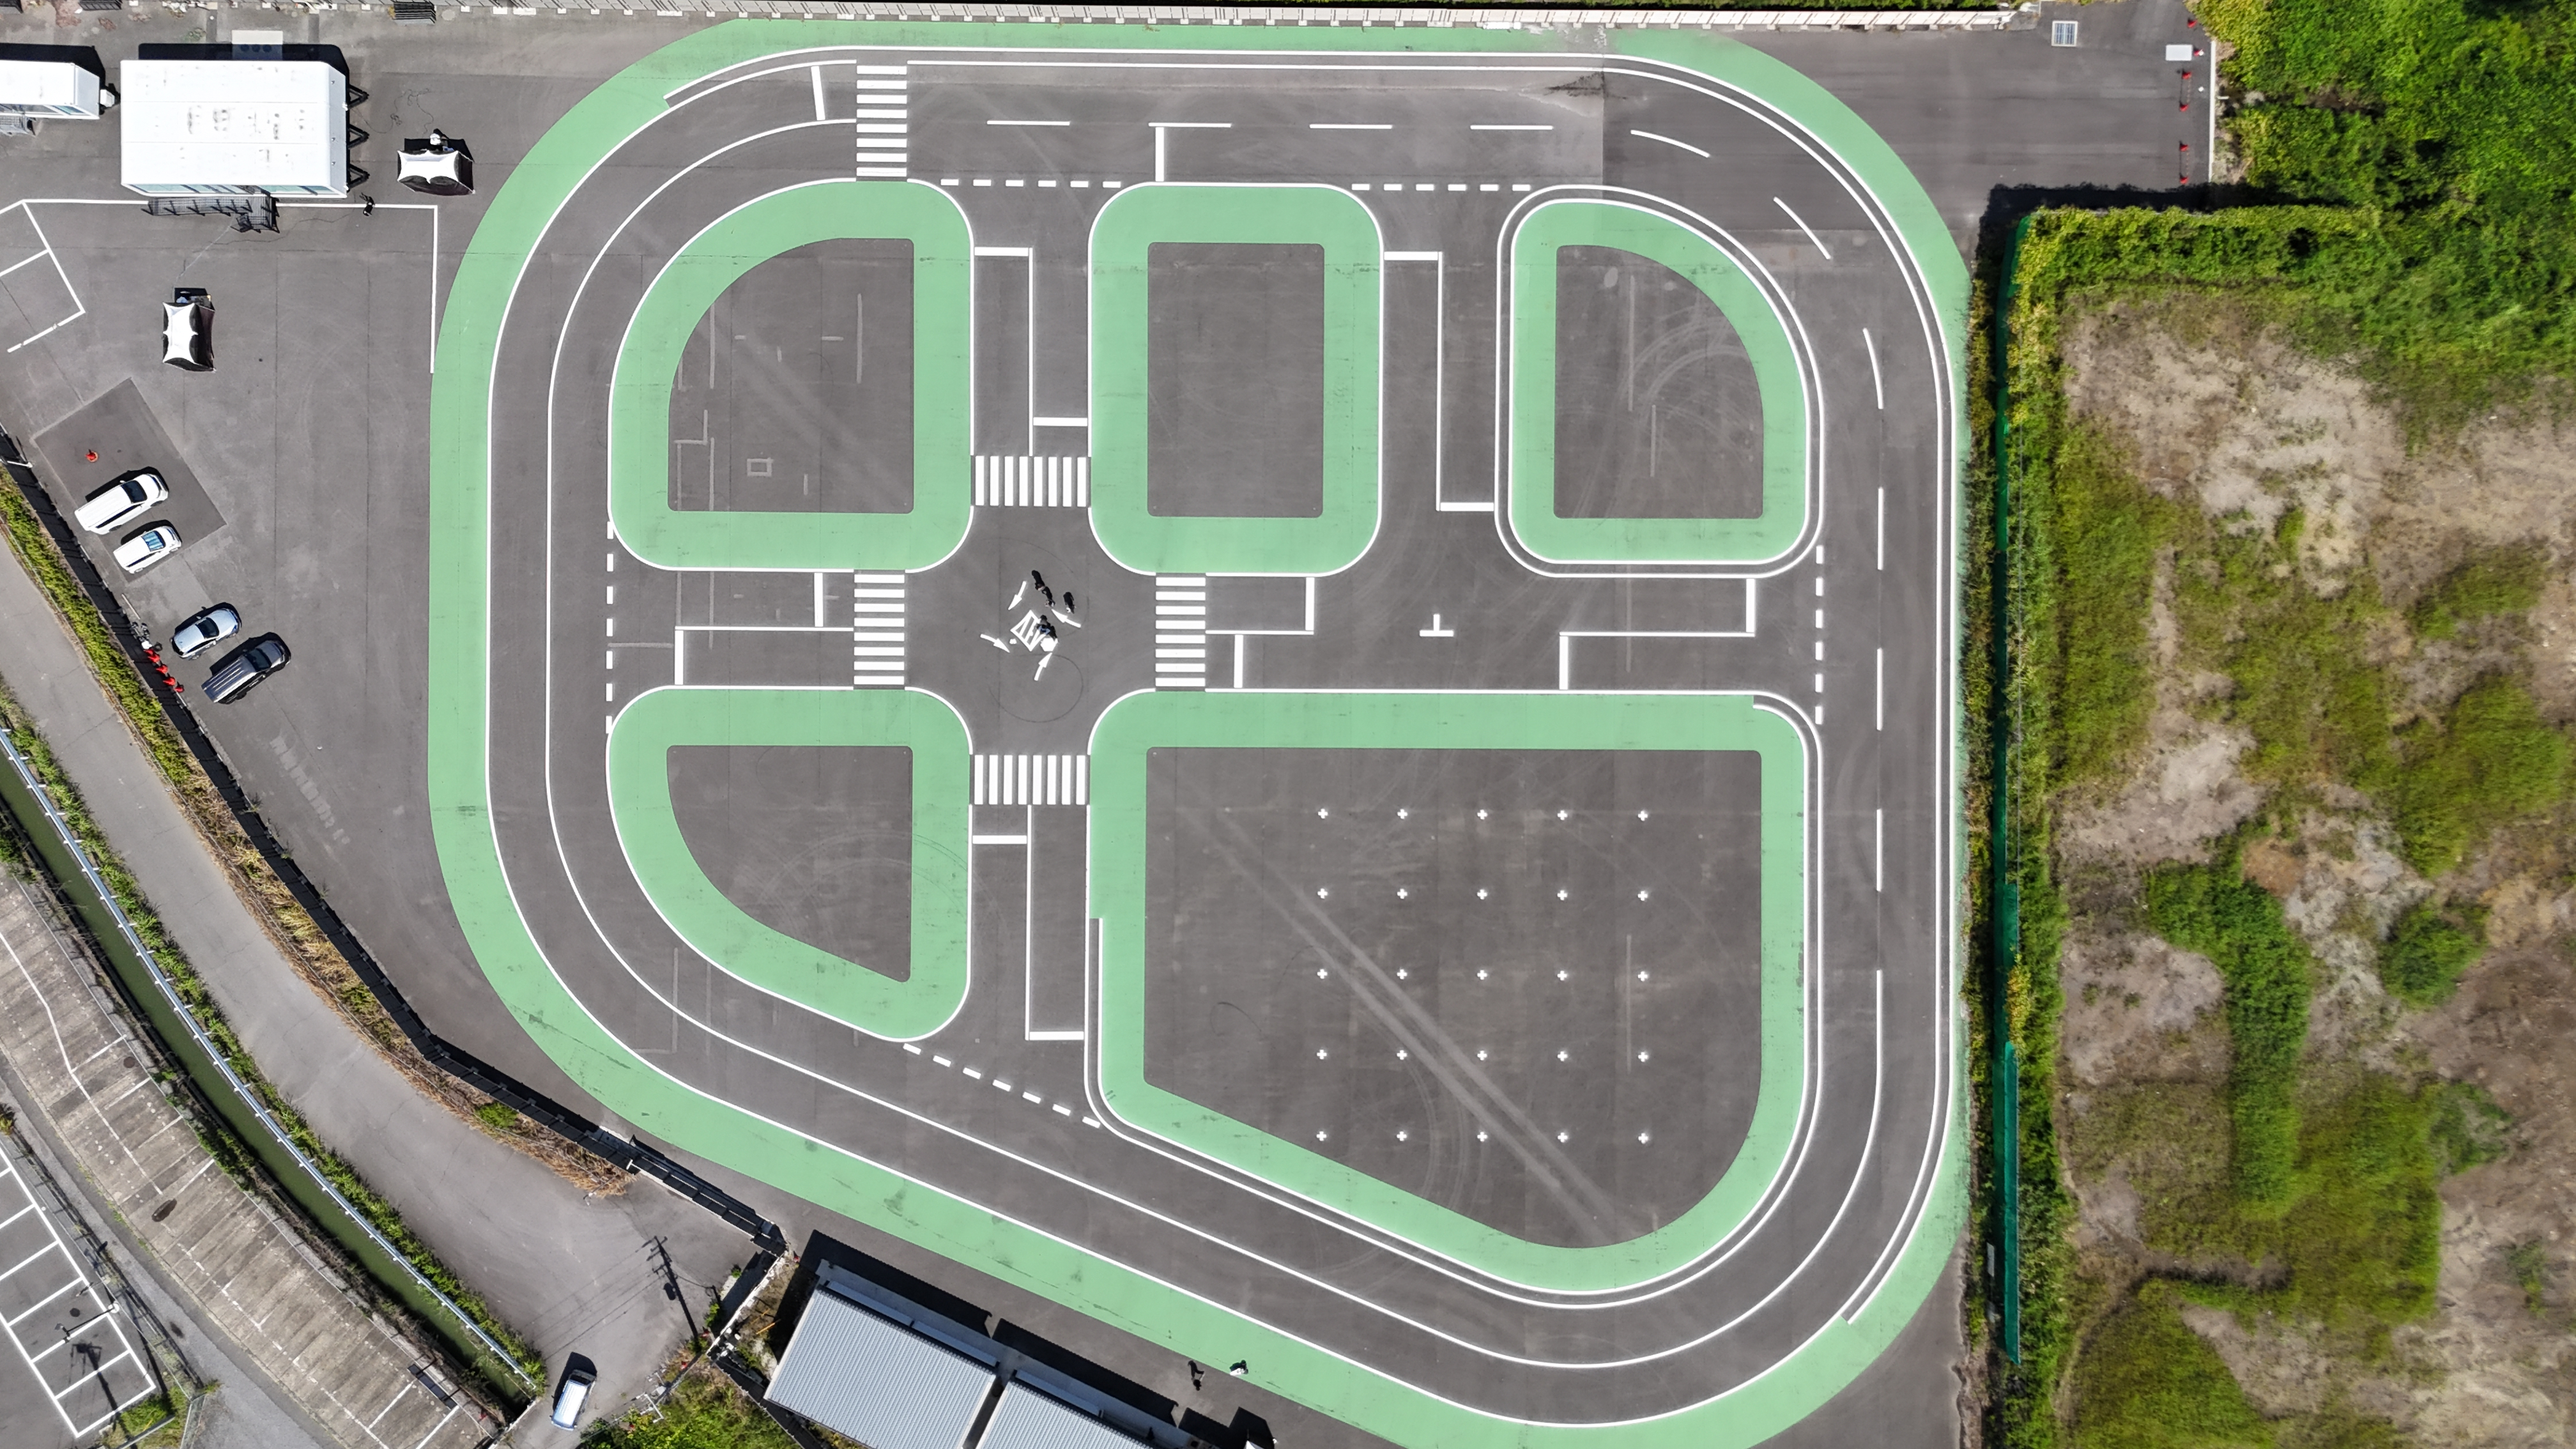
\includegraphics[keepaspectratio, scale=0.1]
      {images/AerialViewAndMobilitysPerspetiveOfTheCourse.png}
 \caption{Aerial view and mobility perspective of the course}
 \label{fig:course}
\end{figure}


\section{目的}
本研究では, 経路追従をするパッケージを開発して評価を行うことで作成した経路追従のパッケージの有効性を実環境で検証することを目的とする.


\section{論文の構成}
本論文は以下のように構成される.
まず, 2章で使用するセンサ構成とシステムの概要を示す.
3章では経路追従する際に使用するアルゴリズムについて述べる.
4章では開発したシステムを用いて経路追従をした際の追従性能の評価をおこなう.
5章では経路追従の実験結果をまとめる.

\newpage

% 2章
\chapter{要素技術}
本章では, 本研究に関連する要素技術を述べる.
%!TEX root = ../thesis.tex

\section{ROS 2}
ROS 2(Robot Operating System versition 2)は, オープンソースのロボットソフトウェアフレームワークであり,
ロボットアプリケーションの開発や実行をサポートするミドルウェアである.
異なるバージョンが存在しているが, 本研究ではROS 2 foxyを主に使用している.

\subsection{RViz2}
RViz2(ROS VIsualization2)はROS 2で提供される三次元ビジュアライゼーションツールであり, 
数値で表されるロボットの座標や各センサのデータを視覚的に表すことができる.

\section{GNSS}
GNSS(Global Navigation Satelite System)は, 
人工衛星を利用して地上の現在位置を計測するためのシステムであり, 
アメリカのGPS, ロシアのGLONASS, ヨーロッパのGalileo, 日本のQGSSなどを総称した衛生測位システムを指す.

\subsection{UTM座標系}
UTM(Universal Transverse Mercator)座標系とは, 全世界を経度6度ごとのゾーンに分けて東回りに番号を付けて規格化したものである.
世界的にも大・中縮尺の図法として採用され, 日本では国土地理院の地形図や地勢図で採用されている.

\begin{figure}[H]
  \centering
 \includegraphics[keepaspectratio, scale=0.7]
      {images/UTMCoordinateSystem.png}
 \caption{UTM Coordinate System(source)}
 \label{fig:purepursuit}
\end{figure}

% AIFormulaの会場となるAIモビリティパークは茨城県常総市にあるため, 54帯のUTM座標系を使用する.

\subsection{ECEF座標系}
ECEF(Earth-Centered, Earth-Fixed)座標系とは, 地理的・直交的な座標系であり, 地球の自転と同期して常時回転している座標系である.

\subsection{測地座標系}
測地座標系とは, 地球上の位置を緯度, 経度, および回転楕円体からの高さで表す座標系である.

\section{IMU}
IMU(Inertial Measurement Unit)は, 
3次元の慣性運動を検出する装置である. 
加速度センサーにより並進運動を検出し, 
ジャイロセンサーにより回転運動を検出することができる.

\newpage
% 3章
\chapter{経路追従に用いるアルゴリズム}
本章では, 経路追従に用いるアルゴリズムについて述べる.
%!TEX root = ../thesis.tex

\section{経路追従}
経路追従(Path following)とは, 経路計画(Path planning)で引いた経路に対してモビリティが経路を追従できるようにモビリティを制御することである.
基本的にはモビリティのモデルと制御アルゴリズムを利用することで, 最終的にモビリティの入力値(ステアリング角度や並進速度)を計算することが目的となる.

\subsection{PurePursuit}
PurePursuitアルゴリズムは, 経路追従アルゴリズムの中で最も基礎的だが, 非常に広く使われているアルゴリズムである.

PurePursuitはFig.3.1に示すように目標経路上(Path)に対して一定距離先の点を目標点(Look Ahead)とし, その点に到達するようなステアリング制御を行う.
目標点に対してモビリティが前進することで, より先の目標点にたどり着くように制御を行うため, 結果的に目標経路に追従する形となる.

\begin{figure}[H]
  \centering
 \includegraphics[keepaspectratio, scale=0.5]
      {images/PurePursuit.png}
 \caption{PurePursuit Algorithm}
 \label{fig:purepursuit}
\end{figure}

\section{経路生成}
経路追従を行うためには, 追従するための目標経路(Path)を設定する必要がある.
自律移動モビリティの開発に置いて目標経路の探索を経路計画と呼び, 重要な問題の一つとされている.
本研究では, 目標経路は予め取得した測地座標系の経緯度で用意されたウェイポイントを結ぶ線形経路として設定している.


\subsection{3次スプライン補間}
本研究で取得する目標経路は, ウェイポイントを結ぶ線形経路として設定している.
設定したウェイポイントが疎らである場合に, 離散的で不連続なウェイポイントから, 滑らかで連続的な経路を生成するために3次スプライン補間が使用される.
% そこで, 3次スプライン補間を行うことで, 用意されたウェイポイント上を繋ぐラインに対して曲線を担保することが可能となる.

3次スプライン補間とは, 複数のサンプル点が与えられた時に, そのサンプル点の間を3次の多項式で近似し, 滑らかに保管する手法である.
Fig.3.2にその様子を示す.

\begin{figure}[H]
     \centering
    \includegraphics[keepaspectratio, scale=0.5]
         {images/splinepath.png}
    \caption{Spline path}
    \label{fig:purepursuit}
\end{figure}


\newpage
% 4章
\capter{システムの要件}
ここでは, 経路追従を行うシステムに求められる要件を示す.
% 5章
\chapter{実験}
% 6章
\chapter{結論}
